\documentclass{article}
\usepackage{graphicx}
\usepackage{float}
\usepackage{amsmath}
\usepackage{pgfplots}
\usepackage{array}
\usepackage[margin=1.5cm]{geometry}
\usepackage{adjustbox}
\usepackage{hyperref}
\usepackage{cite}
\usepackage{listings}
\usepackage{xcolor}
\usepackage{comment}
\usepackage{graphicx}
\usepackage{pdfpages}
\usepackage{enumitem}
\usepackage{pgfplotstable}
\usepackage{booktabs}
\usepackage{adjustbox}
\usepackage{changepage}
\usepackage[utf8]{inputenc}
\lstset{ 
literate= {á}{{\'a}}1 
    {é}{{\'e}}1 
    {í}{{\'i}}1 
    {ó}{{\'o}}1 
    {ú}{{\'u}}1
} 

\hypersetup{
colorlinks=true,
linkcolor=blue,
urlcolor=blue,
}

\pgfplotsset{compat=1.17}
\usepackage[portuguese]{babel}

\definecolor{codegreen}{rgb}{0,0.6,0}
\definecolor{codegray}{rgb}{0.5,0.5,0.5}
\definecolor{codepurple}{rgb}{0.58,0,0.82}
\definecolor{backcolour}{rgb}{0.95,0.95,0.92}

\lstdefinestyle{mystyle}{
    backgroundcolor=\color{backcolour},   
    commentstyle=\color{codegreen},
    keywordstyle=\color{magenta},
    numberstyle=\tiny\color{codegray},
    stringstyle=\color{codepurple},
    basicstyle=\ttfamily\footnotesize,
    breakatwhitespace=false,         
    breaklines=true,                 
    captionpos=b,                    
    keepspaces=true,                 
    numbers=left,                    
    numbersep=5pt,                  
    showspaces=false,                
    showstringspaces=false,
    showtabs=false,                  
    tabsize=2
}

\lstset{style=mystyle}

\title{Trabalho Prático de Análise Numérica}
\author{Alisson Cordeiro e Gabriel Gaspar}
\date{}

\begin{document}

\maketitle

\section{Introdução}
\paragraph{} Este trabalho tem como objetivo apresentar o estudo de Interpolação Polinomial, para a matéria de Análise Númerica, do 3° semestre do curso de Ciência da Computação do Instituto Federal do Paraná - Campus Pinhais. A Interpolação Polinomial é uma técnica utilizada para encontrar um polinômio que passa por um conjunto de pontos dados, permitindo a estimativa de valores intermediários e a análise do comportamento da função.

\section{Problemas conhecidos}
\paragraph{} Alguns problemas conhecidos de interpolação polinomial, são:

\begin{itemize}

    \item \textbf{Fenômeno de Runge}\\
    O fenômeno de Runge ocorre quando usamos polinômios de grau alto para interpolar funções suaves, especialmente com pontos igualmente espaçados. Isso pode causar oscilações grandes nas extremidades da interpolação, resultando em aproximações ruins, mesmo com mais pontos.

    \item \textbf{Instabilidade numérica}\\
    Algoritmos como a eliminação de Gauss podem sofrer com instabilidade numérica, especialmente em presença de números muito grandes ou muito pequenos. Pequenos erros de arredondamento podem se propagar e gerar resultados imprecisos.

    \item \textbf{Complexidade}\\
    O algoritmo apresentado tem complexidade \( O(n^3) \), o que significa que o tempo de execução cresce rapidamente com o aumento de \( n \). Isso o torna pouco eficiente para grandes conjuntos de dados.

\end{itemize}



\section{Código-fonte}
\label{sec:codigofonte1}
\paragraph{} Abaixo está o código-fonte do programa solicitado. De maneira resumida, usando interpolação polinomial, é inserido pontos de uma função específica. Com esses pontos, o programa irá encontrar a função polinomial que passe pelos pontos inseridos. Este programa 
\lstinputlisting[language=c++]{code/interpola.cpp}

\section{Utilização do programa}
\paragraph{} Para compilar e utilizar o programa, foi usado o seguinte código:

\begin{lstlisting}[language=bash]
    g++ -o interpola interpola.cpp
\end{lstlisting}

Para uso do programa, foi usado um arquivo de entrada, contendo os valores necessários, sendo o primeiro valor, a quantidade de pontos conhecidos e o restante sendo os pares ordenados representando os pontos. Um exemplo de entrada está disponível abaixo, em \hyperref[sec:resultados]{Resultados}.

\begin{lstlisting}[language=bash]
    ./interpola < entrada.txt
\end{lstlisting}

A saída do programa está de acordo com as especificações do trabalho, com os valores sendo exibidos em ordem crescente do grau da variável, sendo o primeiro valor referente a \( x^0 \), seguido por \( x^1 \), \( x^2 \), até \( x^{n-1} \).

\section{Resultados}
\label{sec:resultados}
\paragraph{} Usando a tabela abaixo como entrada, o número 5 representa a quantidade de pontos e o resto são os pontos em si. Com isso, o programa retorna a função abaixo da tabela.

\begin{table}[ht!]
\centering
\begin{tabular}{cc}
\multicolumn{2}{c}{5} \\
1   & 2 \\
1.3 & 4.4 \\
1.7 & 4.56 \\
1.9 & 5 \\
2.3 & 7 \\
\end{tabular}
\end{table}

\begin{equation*}
f(x) = -10{,}561661x^4 + 77{,}710623x^3 - 207{,}739316x^2 + 241{,}080037x - 98{,}489683
\end{equation*}

A figura abaixo mostra o gráfico da função interpoladora, com os cinco pontos previamente dados plotados sobre ele para verificar o ajuste:

\begin{figure}[H]
    \centering
    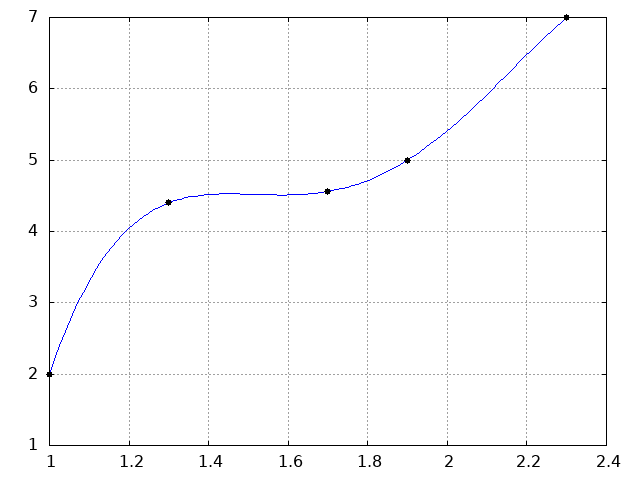
\includegraphics[width=0.5\linewidth]{saida.png}
    \caption{Gráfico da função com os pontos dados previamente}
    \label{fig:saida}
\end{figure}

\section{Exemplos de teste}
\paragraph{} Abaixo estão os três exemplos de teste especificados no documento do trabalho prático.

    \subsection{Exemplo 1}  

        \subsubsection{Entrada do programa}
            \begin{table}[ht!]
            \centering
            \begin{tabular}{cc}
            \multicolumn{2}{c}{6} \\
            -1   & 1 \\
            -0.8 &  1.808704 \\
            0.2 &  0.514624 \\
            0.5 & 0.390625 \\
            1.3 & 0.297649 \\
            2.5 &  15.765625 \\
            \end{tabular}
            \end{table}
        
        \subsubsection{Polinômio interpolador encontrado}
            \begin{align*}
            f(x) &= 0{,}6999999999999992x^5 - 1{,}7099999999999984x^4 + 0{,}4370000000000012x^3 \\
                &\quad + 1{,}6460000000000008x^2 - 1{,}4610000000000005x + 0{,}7399999999999977
            \end{align*}


        \subsubsection{Gráfico dos pontos dados e da função interpoladora}
            \begin{figure}[H]
                \centering
                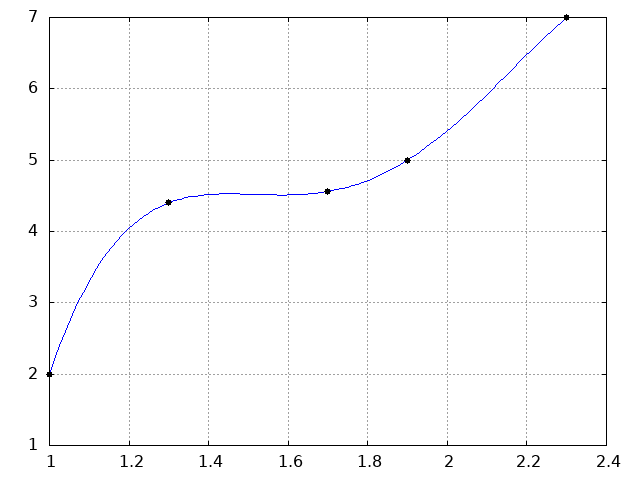
\includegraphics[width=0.5\linewidth]{saida.png}
                \caption{Placeholder}
                \label{fig:placeholder}
            \end{figure}

    \subsection{Exemplo 2}

            \subsubsection{Entrada do programa}
            \begin{table}[ht!]
                \centering
                \begin{tabular}{cc}
                    \multicolumn{2}{c}{4} \\
                    -1   & 3.5 \\
                    -0.8 & 3.25312 \\
                    0.2  & 1.33712 \\
                    0.5  & 0.40625 \\
                \end{tabular}
            \end{table}


            \subsubsection{Polinômio interpolador encontrado}
            \begin{equation*}
                \resizebox{\textwidth}{!}{$
                f(x) = -0{,}2299999999999993x^3 - 0{,}9359999999999992x^2 - 2{,}3580000000000001x + 1{,}8479999999999996
                $}
            \end{equation*}


            \subsubsection{Gráfico dos pontos dados e da função interpoladora}
                \begin{figure}[H]
                    \centering
                    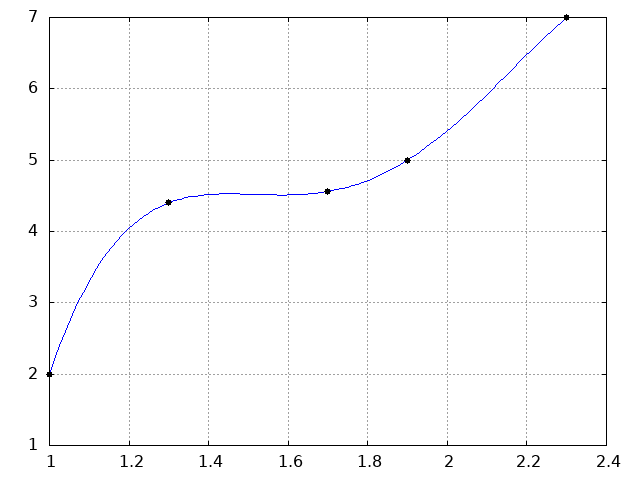
\includegraphics[width=0.5\linewidth]{saida.png}
                    \caption{Placeholder 2}
                    \label{fig:placeholder2}
                \end{figure}

        \subsection{Exemplo 3}

                \subsubsection{Entrada do programa}
                    \begin{table}[ht!]
                        \centering
                        \begin{tabular}{cc}
                            \multicolumn{2}{c}{12} \\
                            2.096564322979868  & 9.745443487783383 \\
                            6.922977157751151  & 1.242846887386261 \\
                            4.220441410259928  & 3.789449024006479 \\
                            1.802878236405755  & 0.8368959365195927 \\
                            1.324377887241789  & 5.936317566366855 \\
                            1.877280316779064  & 9.774407080764629 \\
                            7.557760165820275  & 6.712616033725468 \\
                            4.720106905544402  & 1.230350867632133 \\
                            2.356347202074704  & 8.896870895536257 \\
                            3.905720613358983  & 3.180695896049662 \\
                            2.893813967551298  & 9.832444876731104 \\
                            9.364300979225938  & 0.7215618713442351 \\
                        \end{tabular}
                    \end{table}
                
                \subsubsection{Polinômio interpolador encontrado}
                    \begin{align*}
                    f(x) &= 553846{,}2166198785416782 - 2003336{,}3049126006662846x + 3181893{,}9942112155258656x^2 \\
                        &\quad - 2929693{,}9608184378594160x^3 + 1737428{,}8216584778856486x^4 - 696749{,}3978601371636614x^5 \\
                        &\quad + 192772{,}1912586242251564x^6 - 36792{,}6141283220349578x^7 + 4747{,}0648406829632222x^8 \\
                        &\quad - 394{,}3311612651109499x^9 + 18{,}9837925153810367x^{10} - 0{,}4013836068413766x^{11}
                    \end{align*}

                \subsubsection{Gráfico dos pontos dados e da função interpoladora}
                    \begin{figure}[H]
                        \centering
                        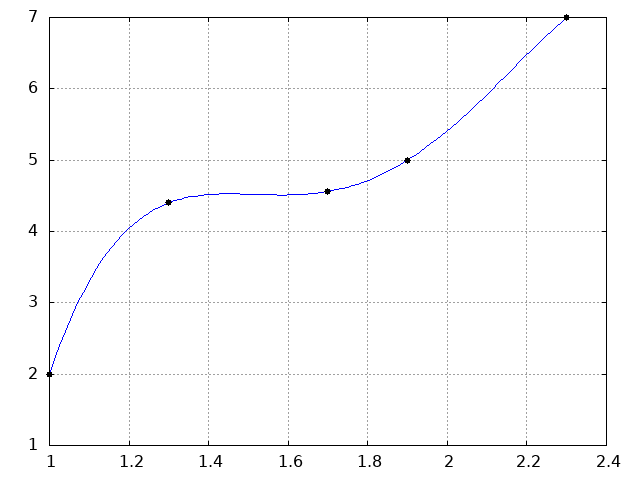
\includegraphics[width=0.5\linewidth]{saida.png}
                        \caption{Placeholder 2}
                        \label{fig:placeholder3}
                    \end{figure}

\newpage
\section{Código-fonte do gerador de gráficos}
\paragraph{} Abaixo está o código-fonte do programa usado para gerar os gráficos. Basicamente, ajustamos o \hyperref[sec:codigofonte1]{programa original} para automaticamente exportar um gráfico com os pontos de entrada e o gráfico da função interpoladora encontrada.

\lstinputlisting[language=c++]{code/coisa.cpp}

\end{document}